\documentclass[11pt]{article}
\title{Meccano pentagons gallery}
\author{https://github.com/heptagons/meccano/penta}
\date{}

%\usepackage{gallery/penta}
%\usepackage{longtable}
\usepackage{../meccano}
\begin{document}

\maketitle
\begin{abstract}
We show constructions of small meccano pentagons from side $12$ to $3$. We restrict all internal strips remain internal and do not overlap.
\end{abstract}

\section{Pentagons of size 12}

\begin{figure}[htp]
 \centering
 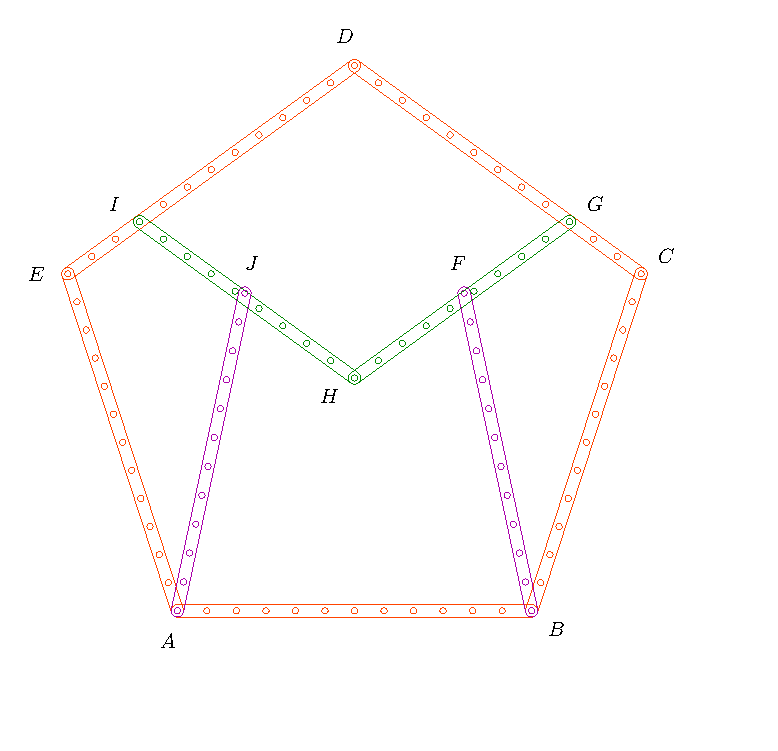
\includegraphics[scale=0.75]{gallery/penta12a}
 \caption{Pentagon size 12.}
 \label{fig:penta12a}
\end{figure}

From figure \ref{fig:penta12a} supose we have a regular pentagon of side 12 $A,B,C,D,E$ and a rhombus $D,I,H,G$ of side $9$. Assume vertice $A$ is at coordinates $(0,0)$ and calculate relative coordinates of vertice $J$. First we calculate the abscissas going through vertices $A,E,I,J$ substracting when we move to the left and adding when we move to the right:
\begin{align}
AJ_x &= AE_x + EI_x + IJ_x\\
 &= -\overline{AE}\cos\left(\frac{2\pi}5\right)
 + \overline{EI}\cos\left(\frac{\pi}5\right) 
 + \overline{IJ}\cos\left(\frac{\pi}5\right)\nonumber\\
 &= -12\left(\frac{\sqrt5 - 1}4\right)
  +3\left(\frac{1+\sqrt5}4\right)
  +4\left(\frac{1+\sqrt5}4\right) = \frac{19-5\sqrt5}4
\end{align}

Then we calculate the ordinates going to the same order of vertices adding when we go up and substracting when we go down:
\begin{align}
AJ_y &= AE_y + EI_y + IJ_y\\
 &= \overline{AE}\sin\left(\frac{2\pi}5\right)
 + \overline{EI}\sin\left(\frac{\pi}5\right) 
 - \overline{IJ}\sin\left(\frac{\pi}5\right)\nonumber\\
 &= 12\left(\frac{\sqrt{10+2\sqrt5}}4\right)
 + 3\left(\frac{\sqrt{10-2\sqrt5}}4\right)
 - 4\left(\frac{\sqrt{10-2\sqrt5}}4\right)\nonumber\\
 &= \frac{12\sqrt{10+2\sqrt5} - \sqrt{10-2\sqrt5}}4 = \frac{\sqrt{1450+190\sqrt5}}4
\end{align}
Finally we calculate the distance $\overline{AJ}$ wich coincides with strip size $11$:
\begin{align}
\overline{AJ} &= \sqrt{(AJ_x)^2 + (AJ_y)^2}\\
 &= \sqrt{\left(\frac{19-5\sqrt5}4\right)^2 + \frac{1450+190\sqrt5}{16}}\nonumber\\
 &= \sqrt{\frac{486-190\sqrt5}{16} + \frac{1450+190\sqrt5}{16}} = \sqrt{121} = 11
\end{align}
\end{document}